\documentclass[dvisvgm]{minimal}

\usepackage{import}
\import{}{figure_layout.tex}

\begin{document}
\scalebox{1.2}{
	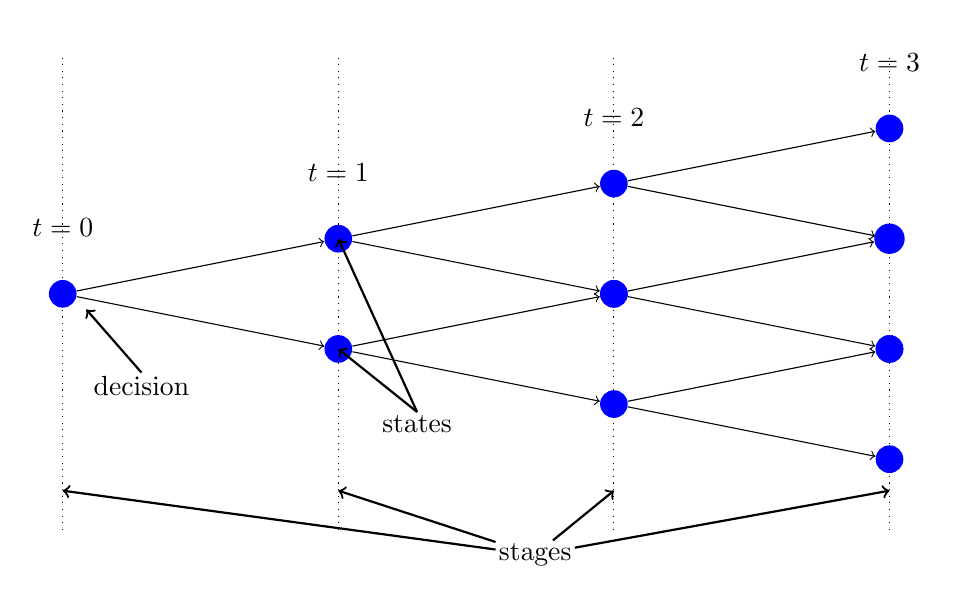
\begin{tikzpicture}[
	                   grow = right,
	edge from parent/.style = {draw,->},
	         label distance = 2mm,
	      every node/.style = {circle, fill=blue, minimum width=1em, inner sep=1pt},
	         level distance = 35mm,
	       sibling distance = 14mm,
	                     ]
	    \draw[dotted] (0,-3) -- (0,3);
		\draw[dotted] (3.5,-3) -- (3.5,3);
		\draw[dotted] (7,-3) -- (7,3);
		\draw[dotted] (10.5,-3) -- (10.5,3);
		\node[label={$t=0$}] (t0) {}
		    child {node {}
		        child {node {}
		            child {node {}}
		            child {node {}}
		                }
		        child {node {}} 
		            }
		    child {node[label={$t=1$}] (t1) {}
		        child {node {}
		            child {node {}} 
		            child {node {0}}
		                }
		        child {node[label={$t=2$}] (t2) {}
		            child {node {}} 
		            child {node[label={$t=3$}] (t3) {}}
		                }
		                };              
		 \draw[->, thick] node[shape=rectangle, fill=none, below] at (1,-1) {decision} (1,-1) -- (0.3,-0.2);
		 \draw[->, thick] node[shape=rectangle, fill=none, below] at (4.5,-1.5) {states} (4.5,-1.5) -- (3.5,0.7);
		 \draw[->, thick] node[shape=rectangle, fill=none, below] at (4.5,-1.5) {} (4.5,-1.5) -- (3.5,-0.7);
		 \draw node[shape=rectangle, fill=none, above] (stages) at (6,-3.5) {stages}; 
		 \draw[->, thick] (stages) -- (0,-2.5);
		 \draw[->, thick] (stages) -- (3.5,-2.5);
		 \draw[->, thick] (stages) -- (7,-2.5);
		 \draw[->, thick] (stages) -- (10.5,-2.5);
	\end{tikzpicture}
	}
\end{document}